\subsection{Benötigte Kenntnisse}
Um das Programm zu erstellen sollten Kenntnisse z.B. für die Capture Compare Unit des Mikrocontrollers vorhanden sein. Die CCU4 hat insgesamt 4 Einheiten und jede einzelne besitzt mehrer Slices von CC40 bis CC43. Slices können untereinander verschachtelt werden um so z.B. Interrupt Service Routinen aufzurufenird, siehe dazu das Reference Manuel.
Der Werte der Register mit denen die Zeit gemessen wird müssen sofort zum beginn der Interrupt Service Routine zwischengespeichert werden damit sichergestellt wird das nicht die Zeit zur Brechung mit gemessen wird.\\

\subsubsection{Durchgeführte Berechnungen}
Auch für die Programmierung waren diverse Berechnungen notwendig. Zur Erzeugung der Ultraschallimpulse wurde ein pulsweitenmoduliertes Rechtecksignal mit einer Frequenz von 40~kHz generiert. Dafür war es notwendig mit Hilfe der CCU4 einen Timer zur erstellen. So musste bei einem Timertakt von 96~MHz eine Periodendauer von 2400 Takten und einem Compare\_Wert von 1200 Takten  konfiguriert werden. Im Zählvorgang des Timers wird der Ausgang nach erreichen des Compare-Wertes auf 1 gesetzt, und nach erreichen der Periodendauer wieder auf 0 zurückgesetzt. Dadurch ergibt sich eine Periodendauer von 25~\textmu s, was einer Frequenz von 40~kHz entspricht.\\
Die Zeit die vergeht bis das Echo des Ultraschall-Impulses zurück kommt wird über einen Timer erfasst. 
\onehalfspacing \\ \\
\(\displaystyle Periodendauer=\frac{96~MHz}{40~kHz} = 2400 \),  \  \  \    \(\displaystyle Compare\_Wert=\frac{2400}{2} = 1200 \) 
\singlespacing


\subsection{Quellcodeentwurf}

\textbf{Programmstruktur:}\\
In der  Distance US main.c befinden sich nur Funktionsaufrufe die eine Grundkonfiguration  für den Controller beinhaltet und eine Schleife die immer wieder abgerufen wird um z.B. eine neue Entfernungsmessung zu starten, siehe Abbildung \ref{fig:main.c1}. Anstatt alles in der Distance US main.c an Programmcode zu verfassen was bei  komplexen Programmen schnell zu Unübersichtlichkeit führt hat das Auslagern den Vorteil das der Quellcode Logisch getrennt werden kann und einer verschlankerung des Codes mit sich bringt. 
Somit stehen in der Main  vor allem die Aufrufe der benötigten Funktionen. 
Auch vereinfacht diese Struktur gerade bei Prototypen das Testen der Funktion. So kann im Falle einer fehlerhaften Funktion einfach der Aufruf auskommentiert werden um zu testen, ob der Fehler wirklich von der Funktion herrührt. Dadurch müssen nicht etliche Zeilen Programmcode der Funktion auskommentiert werden, wodurch schnell Fehler entstehen könnten, durch übriggebliebene Zeichen, oder gar beim entfernen der Auskommentierung gelöschte Zeichen.\\
\begin{minipage}{1\textwidth}
\begin{lstlisting}
#include <stdio.h>
#include <stdbool.h>
#include "bricklib2/logging/logging.h"
#include "bricklib2/bootloader/bootloader.h"
#include "communication.h"
/****Eigene Include Dateien*******/
#include "configs/config.h"
#include "system_timer/system_timer.h"
#include "a16pt.h"
int main(void)
{ 
	logging_init(); 
	logd("Start Distance US V2 Bricklet/n/r");  	//For the Debugmodus
	communication_init(); 					//Function call
	a16pt_init(); 								//Function call	
	while(true)
	{
		a16pt_tick(); 						//Function call
		bootloader_tick(); 					//Function call
		communication_tick(); 				//Function call
		
	}
}
\end{lstlisting}
\captionof{figure}{Die main.c des Distance US}
\label{fig:main.c1}
\end{minipage}\\
Um die Funktionsaufrufe wie die a16pt\_init und die a16pt\_tick zu verstehen muss die Abbildung \ref{fig:a16pt.h}: Headerdatei der a16pt.h näher betrachtet werden.
In der der Datei werden die Funktionen definiert und deren Funktionsanweisung steht dann in der a16pt.c.\\
\begin{minipage}{1\textwidth}
\begin{lstlisting}
#ifndef A16PT_H
#define A16PT_H
#include <stdint.h>
void a16pt_init(void);				//Functional definition
void a16pt_tick(void); 			//Functional definition
uint16_t a16pt_get_distance(void); //Functional definition
#endif
\end{lstlisting}
\captionof{figure}{Headerdatei der a16pt.h}
\label{fig:a16pt.h}
\end{minipage}\\
\\
\textbf{Init Aufruf:}
Auch in der Abbildung \ref{fig:a16pt.c}: Ein Teilausschnitt von der a16pt.c mit den Konfiguration Funktionen werden in der void a16pt-init(void)  weitere Funktionsaufrufe wie z.B. die PWM oder der Externe Interrupt aufgerufen und konfiguriert.

\begin{minipage}{1\textwidth}
\begin{lstlisting}
void a16pt_init(void)
{

/*****************Externe_Interrupt*******************/

	eru_init(eru_port);

/************PWM_Init*****************************/

	XMC_CCU4_Init(CCU41, XMC_CCU4_SLICE_MCMS_ACTION_TRANSFER_PR_CR_PCMP);
	XMC_CCU4_StartPrescaler(CCU41);

	ccu4_pwm_init(pwm_port_0,cc40, period_1);	//P4_4
	ccu4_pwm_set_duty_cycle( cc40, compare_1);

	ccu4_pwm_init(pwm_port_1,cc42, period_0);	//P4_6
	ccu4_pwm_set_duty_cycle( cc42, compare_0);
.
.
.
.
\end{lstlisting}
\captionof{figure}{Ein Teilausschnitt von der a16pt.c mit den Konfiguration Funktionen }
\label{fig:a16pt.c}
\end{minipage}



\textbf{Interrupt Aufruf:}
In der Abbildung \ref{fig:a16pt.c1} :a16pt.c Interrupt Request, werden die für die Entfernungsmessung notwendigen Funktionen und die Interrupt Anweisungen, in dem Fall die IRQ21, abgearbeitet. Außerdem werden die Timer synchron abgeschaltet und aus experimentellen gründen wurde ein weiterer Impuls generiert um zu beobachten wie sich das Nachschwingen bei einer längeren Kurzschlusszeit an der Ultraschallkapsell verhält. Die IRQ wird auch als Interrupt Request bezeichnet und wird von der Hardware oder von der Software ausgelöst.
\\
\begin{minipage}{1\textwidth}
\begin{lstlisting}

/*************Interrupt_Funktionen****************/

void IRQ_Hdlr_21(void) // Compare Interrupt counter 10
{

	// Disable IRQs so we can't be interrupted
	__disable_irq();

	// Set CCU trigger to low, otherwise ccu counter is restarted
	XMC_SCU_SetCcuTriggerLow(XMC_SCU_CCU_TRIGGER_CCU41);

	// Stop slice 2
	XMC_CCU4_SLICE_StopClearTimer(CCU41_CC40);

	// For slice 1 we wait until PWM is run through (to get exactly 10 pwm peaks on P4_4 and P4_6)
	while(XMC_CCU4_SLICE_GetTimerValue(CCU41_CC42) > compare_1) {

		__NOP();
	}
	
	//New pin configuration
	const XMC_GPIO_CONFIG_t pin_out_config	= {
			.mode                = XMC_GPIO_MODE_OUTPUT_PUSH_PULL,
			.output_level        = XMC_GPIO_OUTPUT_LEVEL_HIGH,
		};

	 XMC_GPIO_Init(P4_6, &pin_out_config);
	//Creatw a high impulse
	for(s=0; s<50; s++)
		{
			__NOP();
		}
	// Stop slice 0
	XMC_CCU4_SLICE_StopClearTimer(CCU41_CC42);
	
	//Pin configuration back to the PWM-Mode
	const XMC_GPIO_CONFIG_t gpio_out_config1	= {
		.mode                = XMC_GPIO_MODE_OUTPUT_PUSH_PULL_ALT9,
		.input_hysteresis    = XMC_GPIO_INPUT_HYSTERESIS_STANDARD,
		.output_level        = XMC_GPIO_OUTPUT_LEVEL_LOW,
	};

	XMC_GPIO_Init(P4_6, &gpio_out_config1);
	// Enable IRQs again
	__enable_irq();


}
\end{lstlisting}
\captionof{figure}{Ein Teilausschnitt von der a16pt.c mit einem Interrupt Request}
\label{fig:a16pt.c1}
\end{minipage}

%\newpage
%\begin{minipage}{1\textwidth}Eventuell wo anders hin
%\begin{struktogramm}(120,75)
%\forever
%\assign{\#include aufrufe}
%\while[8]{int main (void)}
 %\sub{Logging init()}
 %\sub{logd ("start Distance us v2 Bricklet")}
 %\sub{Communication init()}
 %\sub{a16pt init()}
%\while[8]{while (1)}
 %\sub{a16pt\_tick()}
 %\sub{bootloader\_tick()}
% \sub{Communication\_tick()}
%\whileend
%\whileend
%\foreverend

%  \ifthenelse{10}{4}{Bedingung 1}{ja}{nein}
%    \ifthenelse{6}{6}{Bedingung 2}{ja}{nein}
%      \assign{Anweisungsblock 1}
%    \change
%      \assign{Anweisungsblock 2}
%    \ifend
%  \change
%    \assign{Anweisungsblock 3}
%  \ifend
%\sub{bla}
%\end{struktogramm}
%\captionof{figure}{Struktogramm der main}\label{fig:Struktogramm der main}
%\end{minipage}

%\newpage
%\begin{figure}[H]
%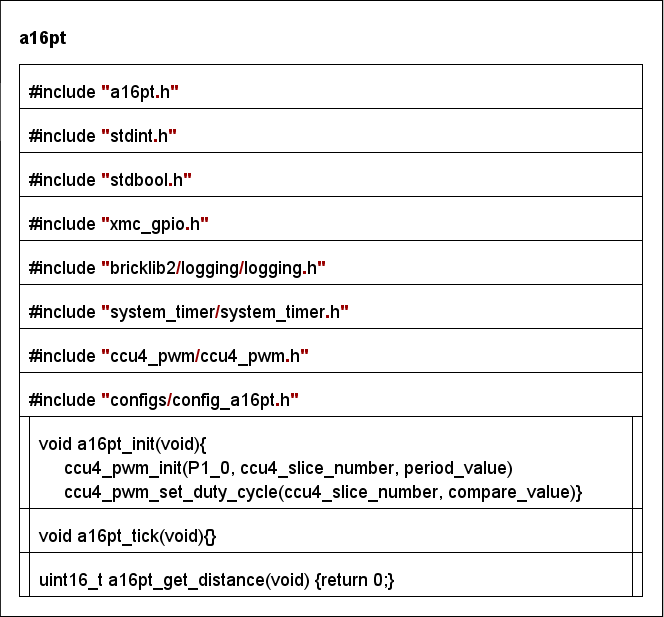
\includegraphics[width=1.0\textwidth]{Struktogramme/a16pt.png}\caption{Struktogramm der a16.pt}\label{fig:Bild2}
%\end{figure}


